Evaluation on Dataset packaged with the respective Libraries:
\subsection{Evaluation on Data from Hand-held Camera}
This set of experiment was conducted inside a well lit room while the camera was focussed on a work desk with multiple common objects. Movement of the camera was smooth and had low velocity. Moreover the frame rate of the camera was 60 frames per second.

\subsubsection{LSD}
As could be seen in Fig. \ref{fig:handheldlsd}, LSD performed very well on the video from handheld camera. It was efficiently able to do the 3D reconstruction and tracking. Check the attached video for th results\footnote{Video at https://youtu.be/Btp6bS0udTA}.

\begin{figure}[H]
	\centering
	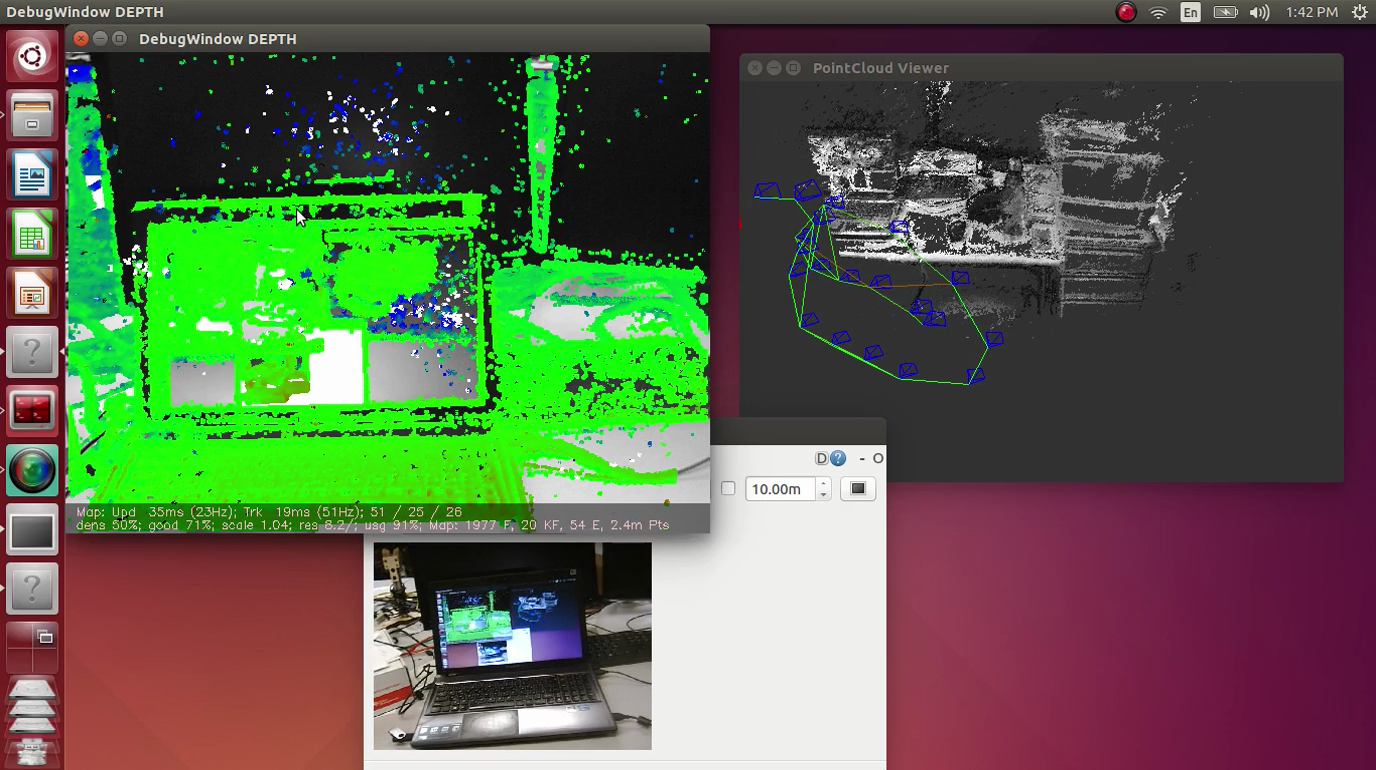
\includegraphics[width=1.0\linewidth]{figures/handHeld_LSD}
	\caption{Snapshot of the off the shelve LSD algorithm implemented using a hand-held camera. The right image shows the keyframes(blue), the trajectory of the camera(green), and the point cloud map at this instance.The left image shows the camera view with the points of the inverse depth map shown in green.}
	\label{fig:handheldlsd}
\end{figure}

\subsubsection{ORB}
For ORB SLAM, initialization is observed using different camera motions. The results are shown in the attached video\footnote{Video at https://youtu.be/1F-ygcA-ZM0\label{xx}}. The initialization time varied with the way camera was moved. If the camera is not moved at all, then it takes around 5.2 seconds to initialize. On the other hand, if we move the camera sideways, the initialization time drops to 3.7 seconds. Interesting thing happened when we do to and fro motion during initialization. To our surprise, the algorithm did not initialize map in this case.

\begin{figure}[H]
	\centering
	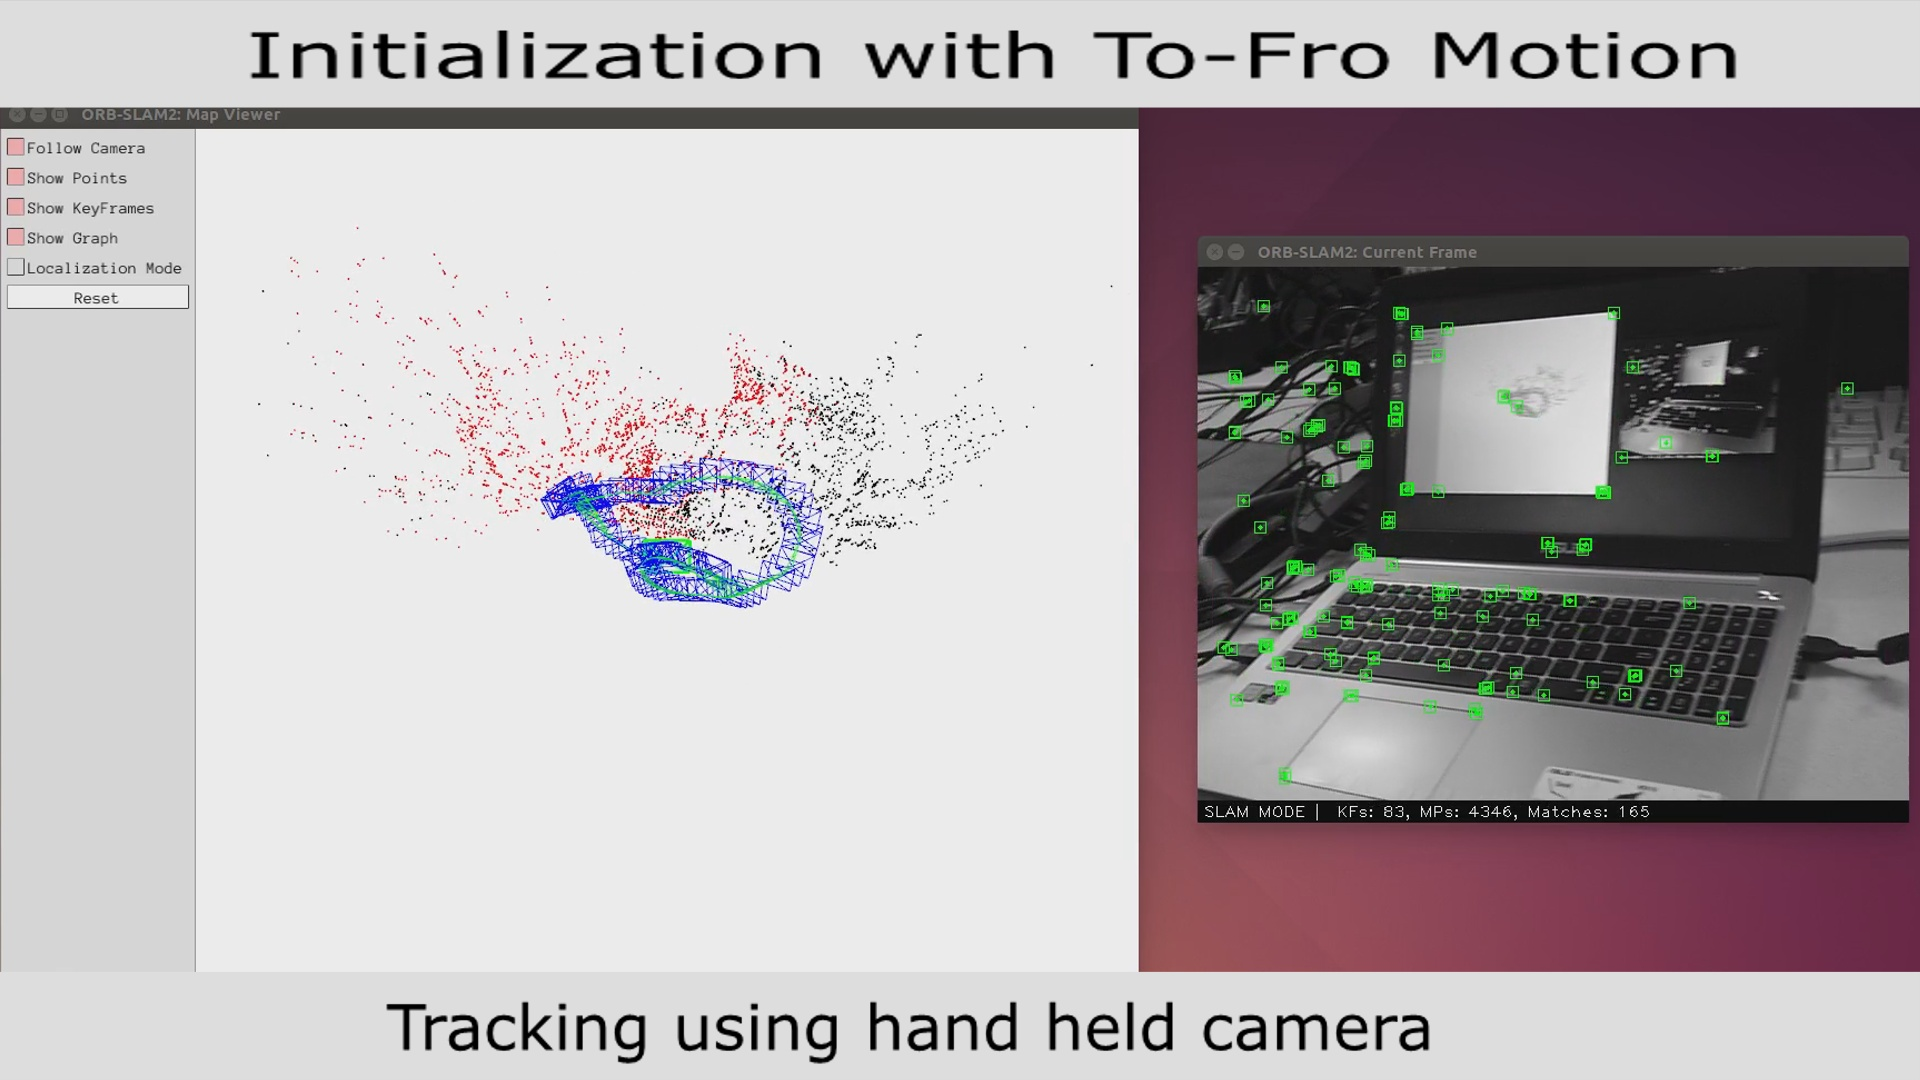
\includegraphics[width=1.0\linewidth]{figures/ORB_handHeld}
	\caption{Snapshot of the off the shelve ORB algorithm implemented using a hand-held camera. The left image shows the keyframes and the point cloud at this instance.The right image shows the camera view with the orb features extracted and shown in green. }
	\label{fig:orbhandheld}
\end{figure}

\subsection{Evaluation on Data from Snake robot}
As mentioned in introduction, the snake moves by pushing the pegs/stones on the ground, and further since the snake’s head moves very close the ground, the video collected from the inbuilt camera in the snake (which is inside its head) majorly contains occlusions by the pegs/stones. In order avoid that and get better video, we mounted a camera over the snake’s head, pointed a little above the horizon. This reduced the issue of high horizon in the image space and occlusion by pegs, although the pegs closer to the camera were still causing occlusion.

\begin{figure}[H]
	\centering
	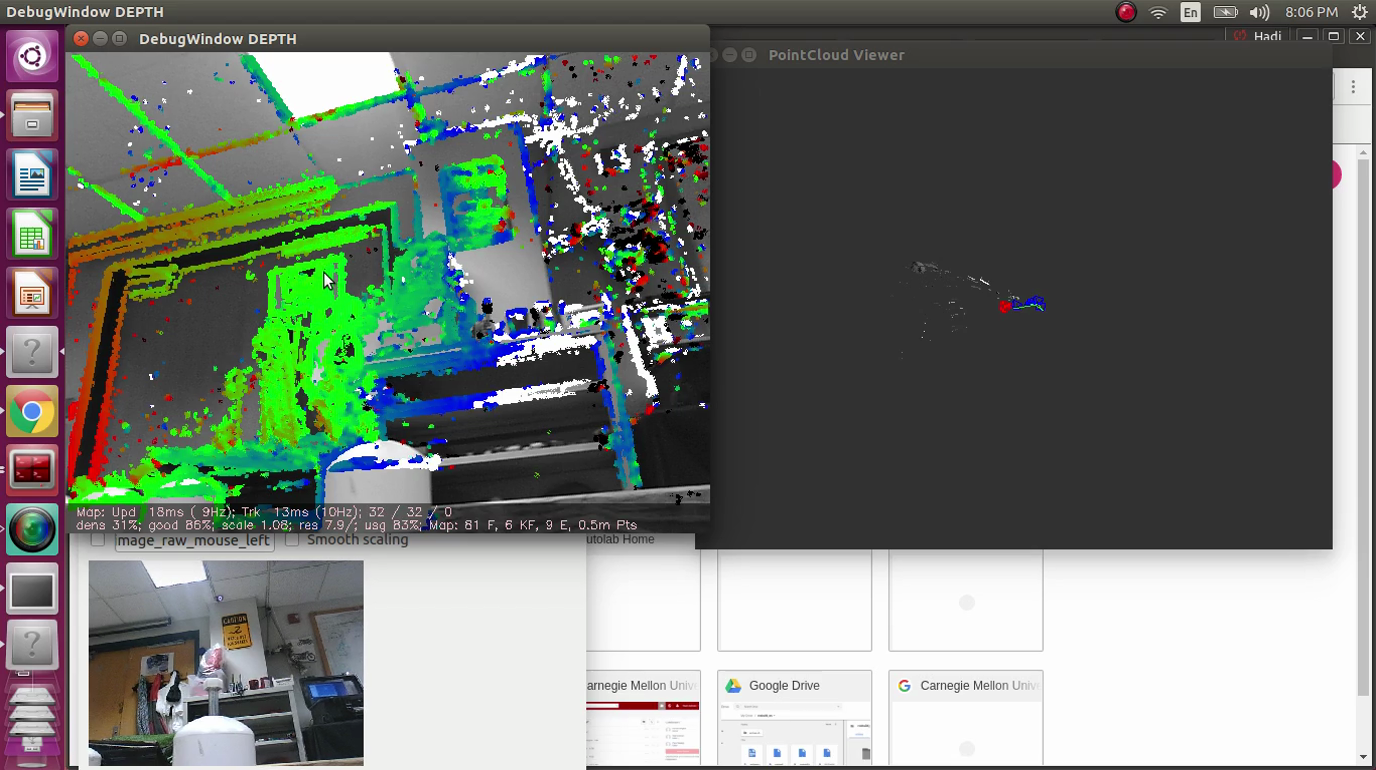
\includegraphics[width=1.0\linewidth]{figures/SNAKE_LSD}
	\caption{Snapshot of the off the shelve LSD algorithm implemented on our Snake robot. The right image shows the keyframes(blue), the trajectory of the camera(green), and the point cloud map at this instance.The left image shows the camera view with the points of the inverse depth map shown in green. As you see in the picture and attached video, the camera looses traking very often due to fast movement of the head of the snake!}
	\label{fig:snakelsd}
\end{figure}
\subsubsection{LSD}
The fast oscillatory and jittery motion of the snake’s head was creating troubles for the LSD. LSD kept loosing the track after every few frames and required initialization as shown in Fig. \ref{fig:snakelsd}. Check the attached video for th results\footnote{Video at https://youtu.be/yBJqJAwULbE}.



\subsubsection{ORB}
It performed better than LSD in terms that it was able to keep track for longer amount of times as shown in Fig. \ref{fig:snakeorb}. During this trial, the truth value of the snake head motion was captured using Opti-track system. The truth value is shown in Fig. \ref{fig:snakerunpscameratrial120170503orb} in blue color. With ORB SLAM, the trajectory derived (scaled by multiplying the coordinates with 10) is as shown in black color in Fig. \ref{fig:snakerunpscameratrial120170503orb}. The difference is quite visible and to our conclusion, the ORB SLAM did not work. We think the reason of failures are: high speed including jerky motions when head gets trapped; some frames with view blocked by pegs resulting in discontinuous tracking; loss of tracking (3 times) during the motion due to poor features. Our proposal going forward is to use high frame rate camera with IMU fusion to recover from loss of tracking and position snake head a little off the ground. Check the attached video for the results\footnote{Video at https://youtu.be/\textunderscore YlEVz5nndY}.

\begin{figure}[H]
	\centering
	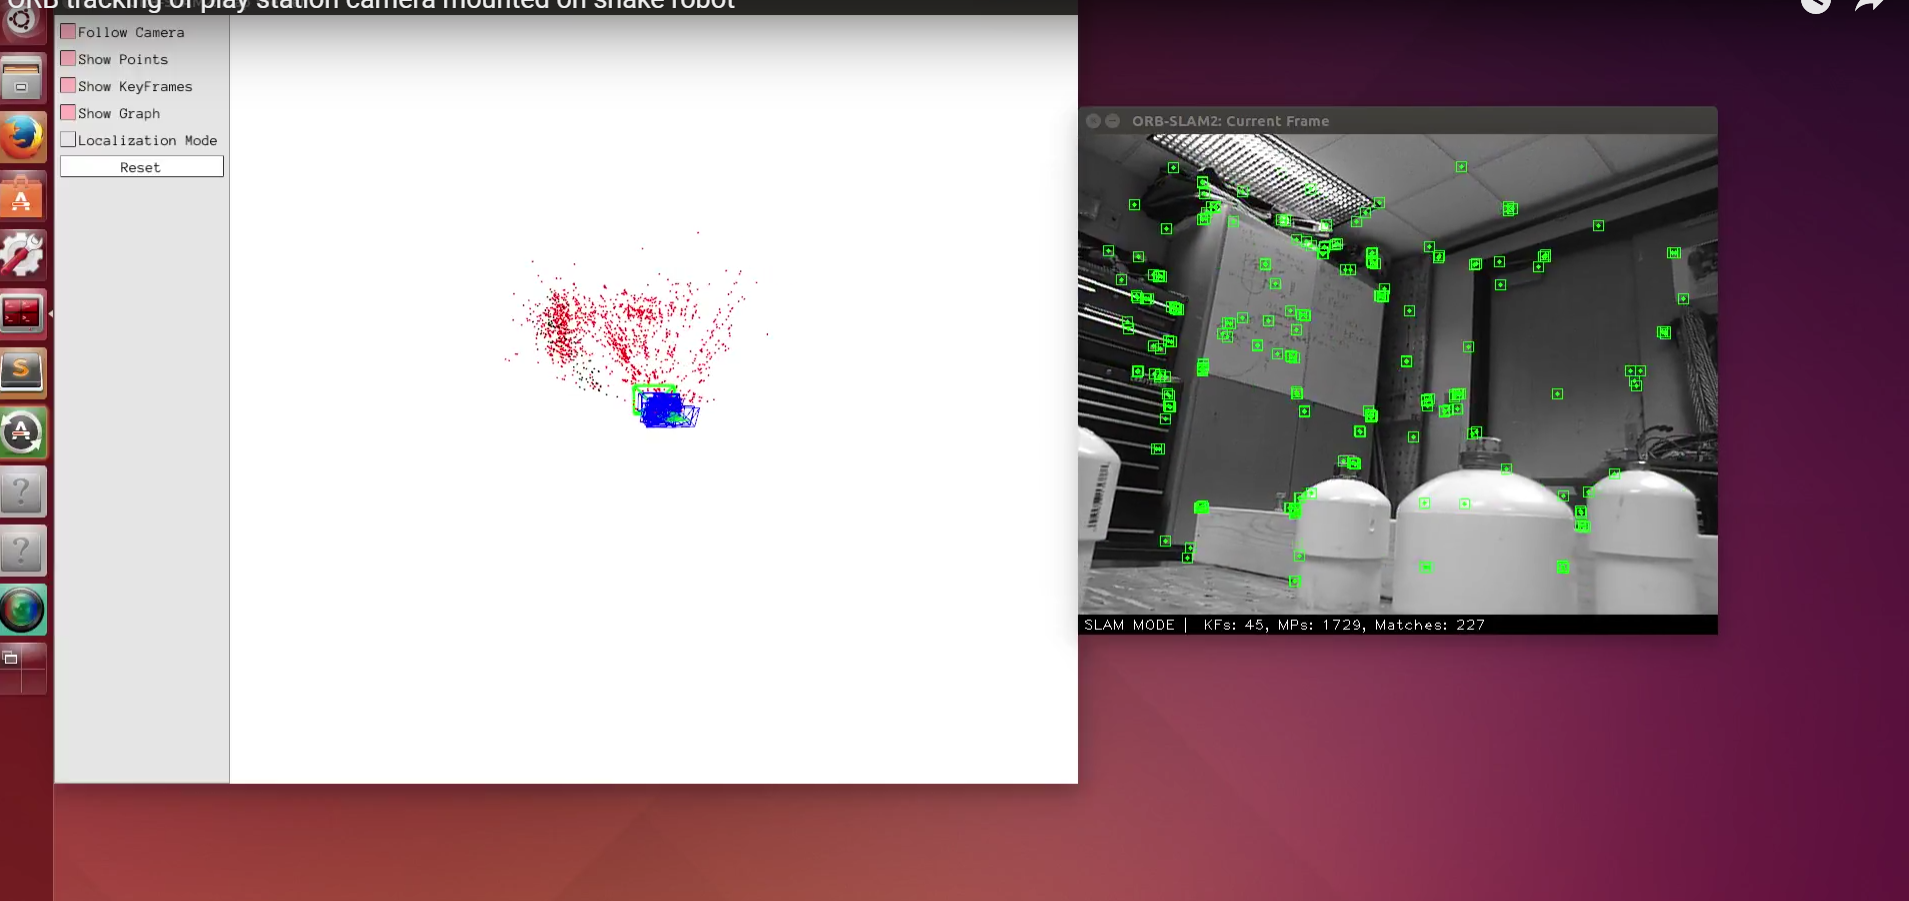
\includegraphics[width=1.0\linewidth]{figures/Snake_ORB}
	\caption{Snapshot of the off the shelve ORB algorithm implemented on our Snake robot. The left image shows the keyframes(blue) and the point cloud map at this instance in red.The right image shows the camera view with the ORB features in green.}
	\label{fig:snakeorb}
\end{figure}

\begin{figure}[H]
	\centering
	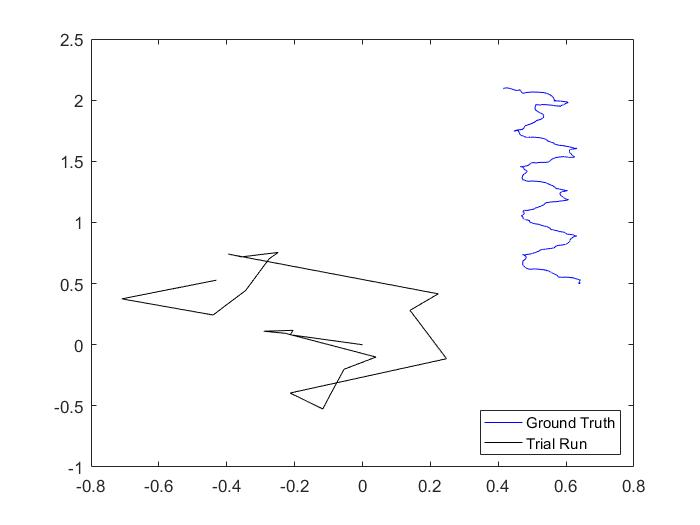
\includegraphics[width=1.0\linewidth]{figures/snakeRun_psCamera_trial1_20170503_ORB}
	\caption{Comparison between the trajectory of the snake robot as obtained by the ORB SLAM algorithm (black) on one hand, and the ground truth captured by a motion capture system (blue) on the other hand.}
	\label{fig:snakerunpscameratrial120170503orb}
\end{figure}

\subsection{Evaluation on Data from Jumping robot}
Unlike the data from the snake mounted camera, the data from jumping robot’s camera does not contain occlusions and high horizon, the only challenge in its data is the jittery or non-smooth motion of the robot.

\subsubsection{LSD}
It worked astonishingly well on the data from jumping robot. It did not loose track, and a snapshot of it could be seen in the Fig. \ref{fig:goatlsd}. Check the attached video for more details \footnote{Video at https://youtu.be/dY85JeTLYEw}
\begin{figure}[H]
	\centering
	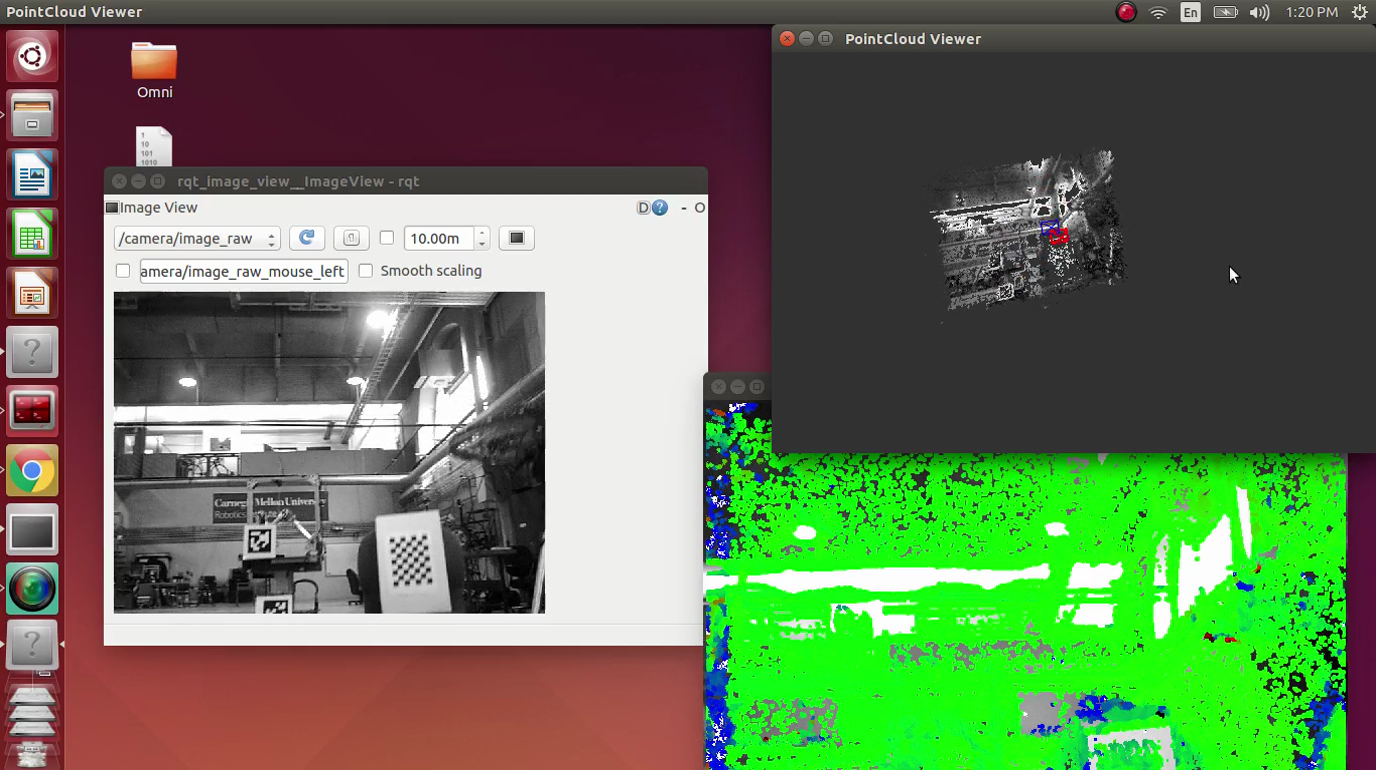
\includegraphics[width=1.0\linewidth]{figures/GOAT_LSD}
	\caption{Snapshot of the off the shelve LSD algorithm implemented on the GOAT robot. The upper right image shows the keyframes(RED) and the point cloud map at this instance in the high bay.The left image shows the camera view, and the lower right image shows the points of the inverse depth map shown in green.}
	\label{fig:goatlsd}
\end{figure}

\subsubsection{ORB}
It was not able to initialize at all on this data. The video was very jittery from the beginning, whereas ORB requires a smoother slow video for initialization

